\section{Register description}
\regover{
{\hyperref[csi-mipi-config]{mipi\_config}}&
\\
\hline
{\hyperref[csi-csi-int-status]{csi\_int\_status}}&
\\
\hline
{\hyperref[csi-csi-int-mask]{csi\_int\_mask}}&
\\
\hline
{\hyperref[csi-csi-int-clear]{csi\_int\_clear}}&
\\
\hline
{\hyperref[csi-csi-int-enable]{csi\_int\_enable}}&
\\
\hline
{\hyperref[csi-gnr-buf-status]{gnr\_buf\_status}}&
\\
\hline
{\hyperref[csi-gnr-buf-rdata]{gnr\_buf\_rdata}}&
\\
\hline
{\hyperref[csi-dphy-config-0]{dphy\_config\_0}}&
\\
\hline
{\hyperref[csi-dphy-config-1]{dphy\_config\_1}}&
\\
\hline
{\hyperref[csi-dphy-config-2]{dphy\_config\_2}}&
\\
\hline
{\hyperref[csi-dphy-config-3]{dphy\_config\_3}}&
\\
\hline
{\hyperref[csi-dphy-config-4]{dphy\_config\_4}}&
\\
\hline
{\hyperref[csi-dphy-config-5]{dphy\_config\_5}}&
\\
\hline
{\hyperref[csi-dummy-reg]{dummy\_reg}}&
\\
\hline
}

\subsection{mipi\_config}
\label{csi-mipi-config}
Address:0x3001a000
 \begin{figure}[H]
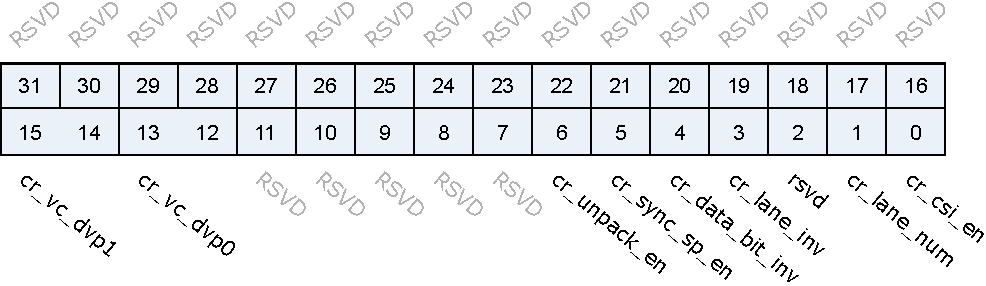
\includegraphics{csi_mipi_config.pdf}
\end{figure}

\regdes{31:16&RSVD& & & \\\hline
15:14&cr\_vc\_dvp1&r/w&2'd1&Virtual Channel number for DVP port 1\\\hline
13:12&cr\_vc\_dvp0&r/w&2'd0&Virtual Channel number for DVP port 0\\\hline
11:7&RSVD& & & \\\hline
6&cr\_unpack\_en&r/w&1'b1&Enable signal for data-unpack function \par 1'b0: Unpack disabled, DVP output is 8-bit valid (byte-in-byte-out) \par 1'b1: Unpack enabled, DVP output format depends on packet data type (RAW 8/10/12/14)
\\\hline
5&cr\_sync\_sp\_en&r/w&1'b0&Enable signal for sync short packets (FS/FE/LS/LE) to be received into gnr\_data\_buf\\\hline
4&cr\_data\_bit\_inv&r/w&1'b0&Controls the bit ordering of PPI I/F data byte, which should be set to little-endian (MSB [7]) \par 1'b0: Not inversed \par 1'b1: Inversed
\\\hline
3&cr\_lane\_inv&r/w&1'b0&Lane inverse \par 1'b0: Lane0 \& Lane1 NOT inversed \par 1'b1: Lane0 \& Lane1 inversed
\\\hline
2&rsvd&rsvd&1'b0&\\\hline
1&cr\_lane\_num&r/w&1'b1&Lane number configuration \par 1'b0: 1-lane MIPI RX \par 1'b1: 2-lane MIPI RX
\\\hline
0&cr\_csi\_en&r/w&1'b0&Enable signal of MIPI receiving function\\\hline

}
\subsection{csi\_int\_status}
\label{csi-csi-int-status}
Address:0x3001a010
 \begin{figure}[H]
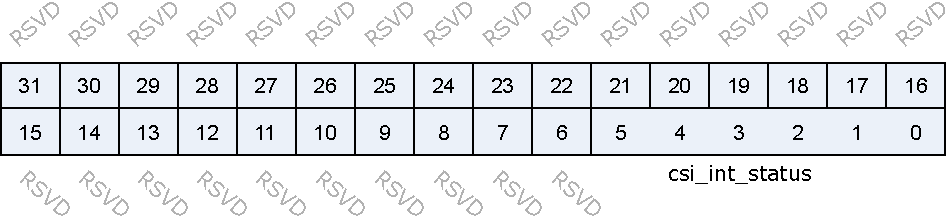
\includegraphics{csi_csi_int_status.pdf}
\end{figure}

\regdes{31:6&RSVD& & & \\\hline
5:0&csi\_int\_status&r&6'h0&[5]: PHY HS SoT Sync Error \par [4]: PHY HS SoT Error \par [3]: CRC Error \par [2]: ECC Error \par [1]: Lane Merging Error \par [0]: Generic Packet Interrupt
\\\hline

}
\subsection{csi\_int\_mask}
\label{csi-csi-int-mask}
Address:0x3001a014
 \begin{figure}[H]
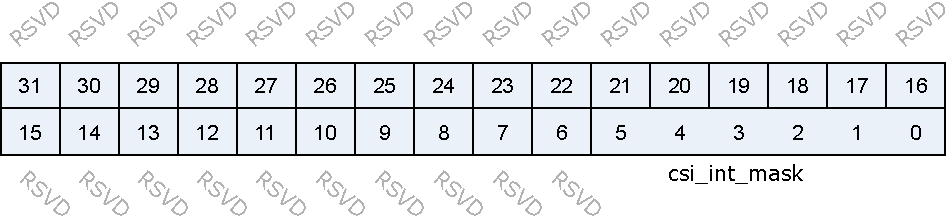
\includegraphics{csi_csi_int_mask.pdf}
\end{figure}

\regdes{31:6&RSVD& & & \\\hline
5:0&csi\_int\_mask&r/w&6'h3F&[5]: PHY HS SoT Sync Error \par [4]: PHY HS SoT Error \par [3]: CRC Error \par [2]: ECC Error \par [1]: Lane Merging Error \par [0]: Generic Packet Interrupt
\\\hline

}
\subsection{csi\_int\_clear}
\label{csi-csi-int-clear}
Address:0x3001a018
 \begin{figure}[H]
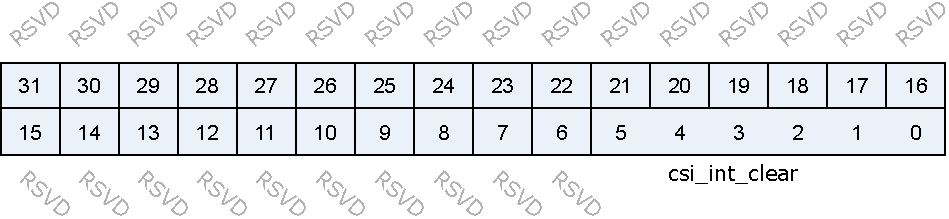
\includegraphics{csi_csi_int_clear.pdf}
\end{figure}

\regdes{31:6&RSVD& & & \\\hline
5:0&csi\_int\_clear&w1p&6'h0&[5]: PHY HS SoT Sync Error \par [4]: PHY HS SoT Error \par [3]: CRC Error \par [2]: ECC Error \par [1]: Lane Merging Error \par [0]: Generic Packet Interrupt
\\\hline

}
\subsection{csi\_int\_enable}
\label{csi-csi-int-enable}
Address:0x3001a01c
 \begin{figure}[H]
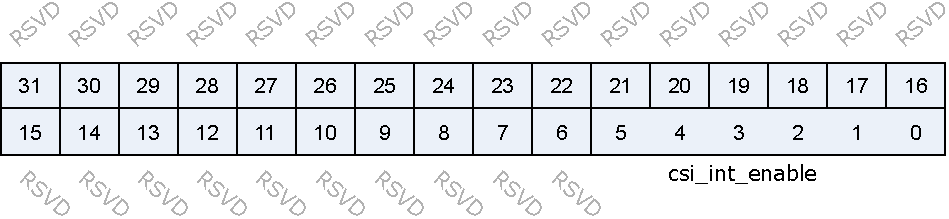
\includegraphics{csi_csi_int_enable.pdf}
\end{figure}

\regdes{31:6&RSVD& & & \\\hline
5:0&csi\_int\_enable&r/w&6'h3F&[5]: PHY HS SoT Sync Error \par [4]: PHY HS SoT Error \par [3]: CRC Error \par [2]: ECC Error \par [1]: Lane Merging Error \par [0]: Generic Packet Interrupt
\\\hline

}
\subsection{gnr\_buf\_status}
\label{csi-gnr-buf-status}
Address:0x3001a020
 \begin{figure}[H]
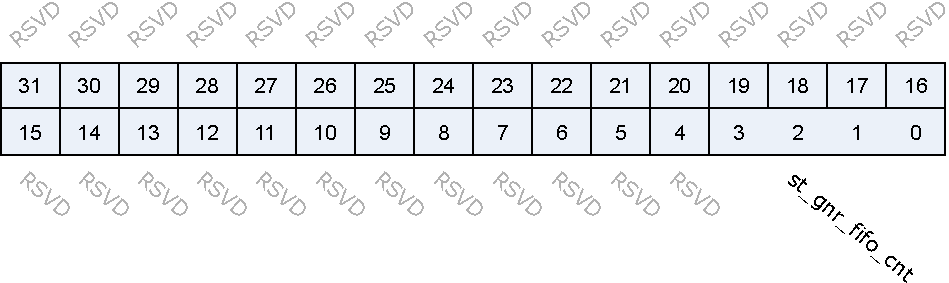
\includegraphics{csi_gnr_buf_status.pdf}
\end{figure}

\regdes{31:4&RSVD& & & \\\hline
3:0&st\_gnr\_fifo\_cnt&r&4'd0&Generic Packet FIFO count\\\hline

}
\subsection{gnr\_buf\_rdata}
\label{csi-gnr-buf-rdata}
Address:0x3001a024
 \begin{figure}[H]
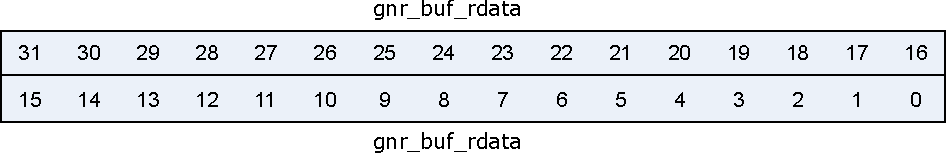
\includegraphics{csi_gnr_buf_rdata.pdf}
\end{figure}

\regdes{31:0&gnr\_buf\_rdata&r&32'h0&Generic Packet FIFO read port\\\hline

}
\subsection{dphy\_config\_0}
\label{csi-dphy-config-0}
Address:0x3001a080
 \begin{figure}[H]
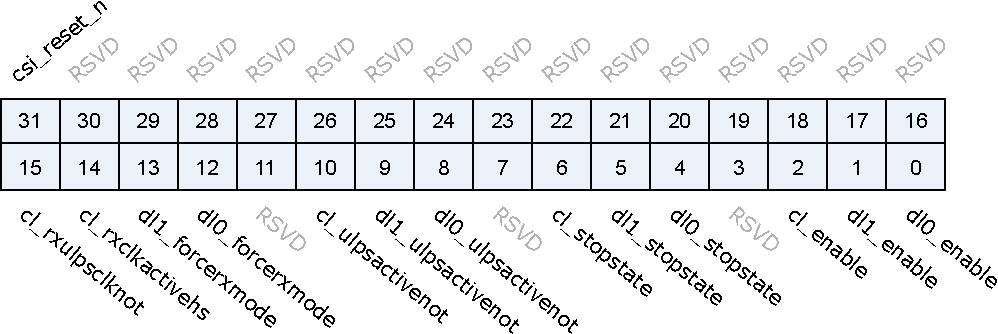
\includegraphics{csi_dphy_config_0.pdf}
\end{figure}

\regdes{31&csi\_reset\_n&r/w&1'b0&MIPI CSI D-PHY reset pin\\\hline
30:16&RSVD& & & \\\hline
15&cl\_rxulpsclknot&r&1'b1&Receiver Ultra-Low Power State on clock lane\\\hline
14&cl\_rxclkactivehs&r&1'b0&Receiver clock active\\\hline
13&dl1\_forcerxmode&r/w&1'b0&Force Lane1 to Re-Initialize\\\hline
12&dl0\_forcerxmode&r/w&1'b0&Force Lane0 to Re-Initialize\\\hline
11&RSVD& & & \\\hline
10&cl\_ulpsactivenot&r&1'b1&Clock lane is NOT in the ULP state\\\hline
9&dl1\_ulpsactivenot&r&1'b1&Data lane1 is NOT in the ULP state\\\hline
8&dl0\_ulpsactivenot&r&1'b1&Data lane0 is NOT in the ULP state\\\hline
7&RSVD& & & \\\hline
6&cl\_stopstate&r&1'b1&Clock lane is in Stop state\\\hline
5&dl1\_stopstate&r&1'b1&Data lane1 is in Stop state\\\hline
4&dl0\_stopstate&r&1'b1&Data lane0 is in Stop state\\\hline
3&RSVD& & & \\\hline
2&cl\_enable&r/w&1'b0&Clock lane enable\\\hline
1&dl1\_enable&r/w&1'b0&Data lane1 enable\\\hline
0&dl0\_enable&r/w&1'b0&Data lane0 enable\\\hline

}
\subsection{dphy\_config\_1}
\label{csi-dphy-config-1}
Address:0x3001a084
 \begin{figure}[H]
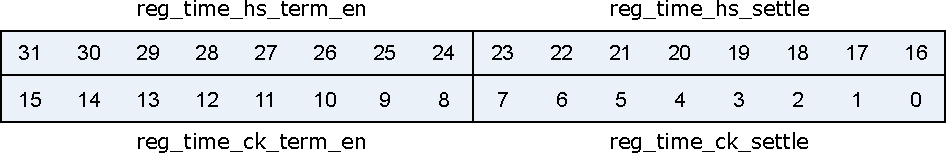
\includegraphics{csi_dphy_config_1.pdf}
\end{figure}

\regdes{31:24&reg\_time\_hs\_term\_en&r/w&8'hF&MIPI CSI D-PHY control register - reg\_time\_hs\_term\_en (2x T\_datarate), txclkesc: 40M, datarate: 800Mbps\\\hline
23:16&reg\_time\_hs\_settle&r/w&8'h2F&MIPI CSI D-PHY control register - reg\_time\_hs\_settle (2x T\_datarate)\\\hline
15:8&reg\_time\_ck\_term\_en&r/w&8'h1&MIPI CSI D-PHY control register - reg\_time\_ck\_term\_en (tx\_clk\_esc)\\\hline
7:0&reg\_time\_ck\_settle&r/w&8'h0A&MIPI CSI D-PHY control register - reg\_time\_ck\_settle (tx\_clk\_esc)\\\hline

}
\subsection{dphy\_config\_2}
\label{csi-dphy-config-2}
Address:0x3001a088
 \begin{figure}[H]
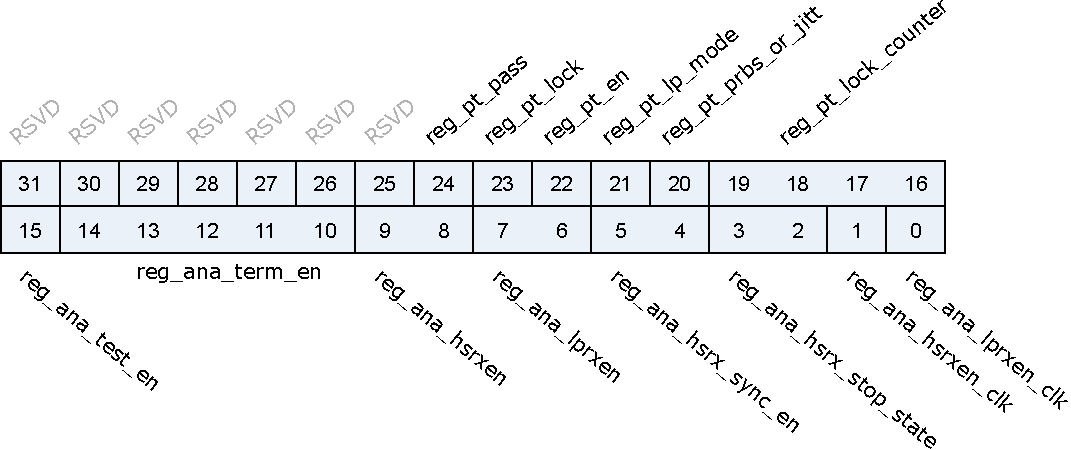
\includegraphics{csi_dphy_config_2.pdf}
\end{figure}

\regdes{31:25&RSVD& & & \\\hline
24&reg\_pt\_pass&r&1'b0&MIPI CSI D-PHY control register - reg\_pt\_pass\\\hline
23&reg\_pt\_lock&r&1'b0&MIPI CSI D-PHY control register - reg\_pt\_lock\\\hline
22&reg\_pt\_en&r/w&1'b0&MIPI CSI D-PHY control register - reg\_pt\_en\\\hline
21&reg\_pt\_lp\_mode&r/w&1'b0&MIPI CSI D-PHY control register - reg\_pt\_lp\_mode\\\hline
20&reg\_pt\_prbs\_or\_jitt&r/w&1'b0&MIPI CSI D-PHY control register - reg\_pt\_prbs\_or\_jitt\\\hline
19:16&reg\_pt\_lock\_counter&r/w&4'h0&MIPI CSI D-PHY control register - reg\_pt\_lock\_counter\\\hline
15&reg\_ana\_test\_en&r/w&1'b0&MIPI CSI D-PHY control register - reg\_ana\_test\_en\\\hline
14:10&reg\_ana\_term\_en&r/w&5'h0&MIPI CSI D-PHY control register - reg\_ana\_term\_en\\\hline
9:8&reg\_ana\_hsrxen&r/w&2'b00&MIPI CSI D-PHY control register - reg\_ana\_hsrxen\\\hline
7:6&reg\_ana\_lprxen&r/w&2'b00&MIPI CSI D-PHY control register - reg\_ana\_lprxen\\\hline
5:4&reg\_ana\_hsrx\_sync\_en&r/w&2'b00&MIPI CSI D-PHY control register - reg\_ana\_hsrx\_sync\_en\\\hline
3:2&reg\_ana\_hsrx\_stop\_state&r/w&2'b00&MIPI CSI D-PHY control register - reg\_ana\_hsrx\_stop\_state\\\hline
1&reg\_ana\_hsrxen\_clk&r/w&1'b0&MIPI CSI D-PHY control register - reg\_ana\_hsrxen\_clk\\\hline
0&reg\_ana\_lprxen\_clk&r/w&1'b0&MIPI CSI D-PHY control register - reg\_ana\_lprxen\_clk\\\hline

}
\subsection{dphy\_config\_3}
\label{csi-dphy-config-3}
Address:0x3001a08c
 \begin{figure}[H]
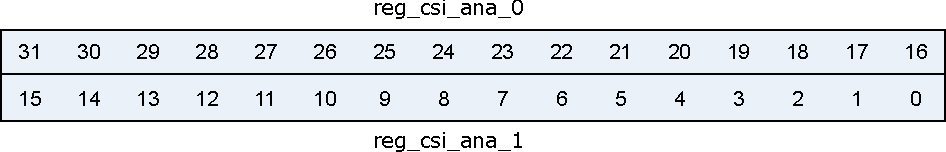
\includegraphics{csi_dphy_config_3.pdf}
\end{figure}

\regdes{31:16&reg\_csi\_ana\_0&r/w&16'h0000&MIPI CSI D-PHY control register - reg\_csi\_ana\_0\\\hline
15:0&reg\_csi\_ana\_1&r/w&16'h0000&MIPI CSI D-PHY control register - reg\_csi\_ana\_1\\\hline

}
\subsection{dphy\_config\_4}
\label{csi-dphy-config-4}
Address:0x3001a090
 \begin{figure}[H]
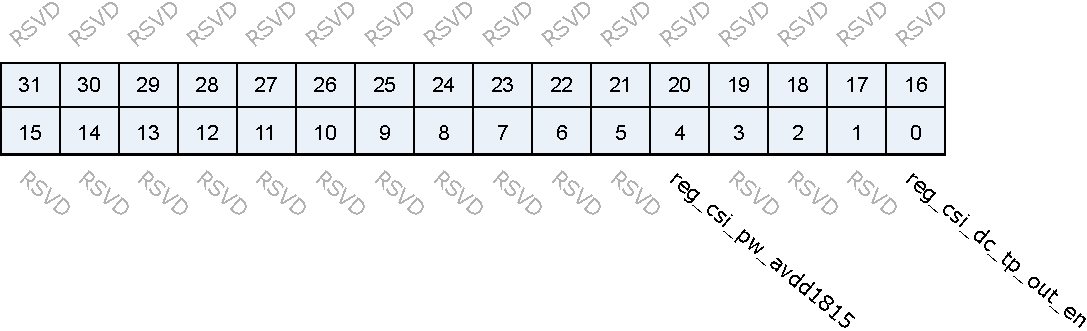
\includegraphics{csi_dphy_config_4.pdf}
\end{figure}

\regdes{31:5&RSVD& & & \\\hline
4&reg\_csi\_pw\_avdd1815&r/w&1'b0&0: power switch on\\\hline
3:1&RSVD& & & \\\hline
0&reg\_csi\_dc\_tp\_out\_en&r/w&1'b0&\\\hline

}
\subsection{dphy\_config\_5}
\label{csi-dphy-config-5}
Address:0x3001a094
 \begin{figure}[H]
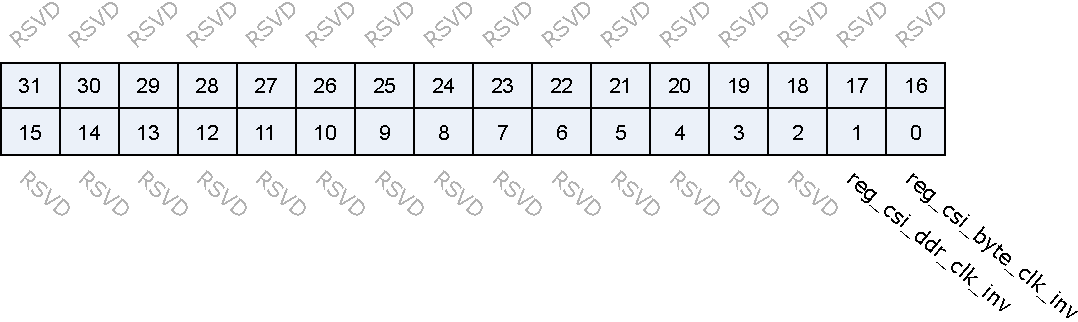
\includegraphics{csi_dphy_config_5.pdf}
\end{figure}

\regdes{31:2&RSVD& & & \\\hline
1&reg\_csi\_ddr\_clk\_inv&r/w&1'b0&\\\hline
0&reg\_csi\_byte\_clk\_inv&r/w&1'b0&\\\hline

}
\subsection{dummy\_reg}
\label{csi-dummy-reg}
Address:0x3001a0fc
 \begin{figure}[H]
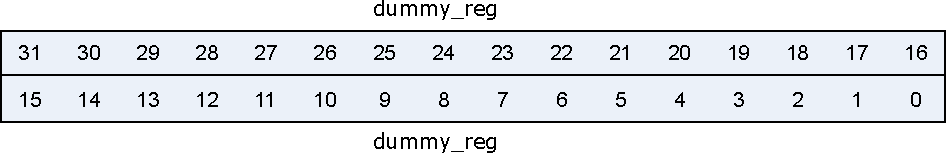
\includegraphics{csi_dummy_reg.pdf}
\end{figure}

\regdes{31:0&dummy\_reg&r/w&32'h0&Dummy registers\\\hline

}
